\documentclass[twoside]{book}

% Packages required by doxygen
\usepackage{fixltx2e}
\usepackage{calc}
\usepackage{doxygen}
\usepackage[export]{adjustbox} % also loads graphicx
\usepackage{graphicx}
\usepackage[utf8]{inputenc}
\usepackage{makeidx}
\usepackage{multicol}
\usepackage{multirow}
\PassOptionsToPackage{warn}{textcomp}
\usepackage{textcomp}
\usepackage[nointegrals]{wasysym}
\usepackage[table]{xcolor}

% Font selection
\usepackage[T1]{fontenc}
\usepackage[scaled=.90]{helvet}
\usepackage{courier}
\usepackage{amssymb}
\usepackage{sectsty}
\renewcommand{\familydefault}{\sfdefault}
\allsectionsfont{%
  \fontseries{bc}\selectfont%
  \color{darkgray}%
}
\renewcommand{\DoxyLabelFont}{%
  \fontseries{bc}\selectfont%
  \color{darkgray}%
}
\newcommand{\+}{\discretionary{\mbox{\scriptsize$\hookleftarrow$}}{}{}}

% Page & text layout
\usepackage{geometry}
\geometry{%
  a4paper,%
  top=2.5cm,%
  bottom=2.5cm,%
  left=2.5cm,%
  right=2.5cm%
}
\tolerance=750
\hfuzz=15pt
\hbadness=750
\setlength{\emergencystretch}{15pt}
\setlength{\parindent}{0cm}
\setlength{\parskip}{3ex plus 2ex minus 2ex}
\makeatletter
\renewcommand{\paragraph}{%
  \@startsection{paragraph}{4}{0ex}{-1.0ex}{1.0ex}{%
    \normalfont\normalsize\bfseries\SS@parafont%
  }%
}
\renewcommand{\subparagraph}{%
  \@startsection{subparagraph}{5}{0ex}{-1.0ex}{1.0ex}{%
    \normalfont\normalsize\bfseries\SS@subparafont%
  }%
}
\makeatother

% Headers & footers
\usepackage{fancyhdr}
\pagestyle{fancyplain}
\fancyhead[LE]{\fancyplain{}{\bfseries\thepage}}
\fancyhead[CE]{\fancyplain{}{}}
\fancyhead[RE]{\fancyplain{}{\bfseries\leftmark}}
\fancyhead[LO]{\fancyplain{}{\bfseries\rightmark}}
\fancyhead[CO]{\fancyplain{}{}}
\fancyhead[RO]{\fancyplain{}{\bfseries\thepage}}
\fancyfoot[LE]{\fancyplain{}{}}
\fancyfoot[CE]{\fancyplain{}{}}
\fancyfoot[RE]{\fancyplain{}{\bfseries\scriptsize Generated by Doxygen }}
\fancyfoot[LO]{\fancyplain{}{\bfseries\scriptsize Generated by Doxygen }}
\fancyfoot[CO]{\fancyplain{}{}}
\fancyfoot[RO]{\fancyplain{}{}}
\renewcommand{\footrulewidth}{0.4pt}
\renewcommand{\chaptermark}[1]{%
  \markboth{#1}{}%
}
\renewcommand{\sectionmark}[1]{%
  \markright{\thesection\ #1}%
}

% Indices & bibliography
\usepackage{natbib}
\usepackage[titles]{tocloft}
\setcounter{tocdepth}{3}
\setcounter{secnumdepth}{5}
\makeindex

% Hyperlinks (required, but should be loaded last)
\usepackage{ifpdf}
\ifpdf
  \usepackage[pdftex,pagebackref=true]{hyperref}
\else
  \usepackage[ps2pdf,pagebackref=true]{hyperref}
\fi
\hypersetup{%
  colorlinks=true,%
  linkcolor=blue,%
  citecolor=blue,%
  unicode%
}

% Custom commands
\newcommand{\clearemptydoublepage}{%
  \newpage{\pagestyle{empty}\cleardoublepage}%
}

\usepackage{caption}
\captionsetup{labelsep=space,justification=centering,font={bf},singlelinecheck=off,skip=4pt,position=top}

%===== C O N T E N T S =====

\begin{document}

% Titlepage & ToC
\hypersetup{pageanchor=false,
             bookmarksnumbered=true,
             pdfencoding=unicode
            }
\pagenumbering{alph}
\begin{titlepage}
\vspace*{7cm}
\begin{center}%
{\Large Multi Ego Plugin \\[1ex]\large 01 }\\
\vspace*{1cm}
{\large Generated by Doxygen 1.8.13}\\
\end{center}
\end{titlepage}
\clearemptydoublepage
\pagenumbering{roman}
\tableofcontents
\clearemptydoublepage
\pagenumbering{arabic}
\hypersetup{pageanchor=true}

%--- Begin generated contents ---
\chapter{Hierarchical Index}
\section{Class Hierarchy}
This inheritance list is sorted roughly, but not completely, alphabetically\+:\begin{DoxyCompactList}
\item Dynamics\+Plugin\begin{DoxyCompactList}
\item \contentsline{section}{Module\+:\+:Multi\+Ego}{\pageref{classModule_1_1MultiEgo}}{}
\end{DoxyCompactList}
\end{DoxyCompactList}

\chapter{Class Index}
\section{Class List}
Here are the classes, structs, unions and interfaces with brief descriptions\+:\begin{DoxyCompactList}
\item\contentsline{section}{\hyperlink{classModule_1_1MultiEgo}{Module\+::\+Multi\+Ego} }{\pageref{classModule_1_1MultiEgo}}{}
\end{DoxyCompactList}

\chapter{Class Documentation}
\hypertarget{classModule_1_1MultiEgo}{}\section{Module\+:\+:Multi\+Ego Class Reference}
\label{classModule_1_1MultiEgo}\index{Module\+::\+Multi\+Ego@{Module\+::\+Multi\+Ego}}


Inheritance diagram for Module\+:\+:Multi\+Ego\+:\nopagebreak
\begin{figure}[H]
\begin{center}
\leavevmode
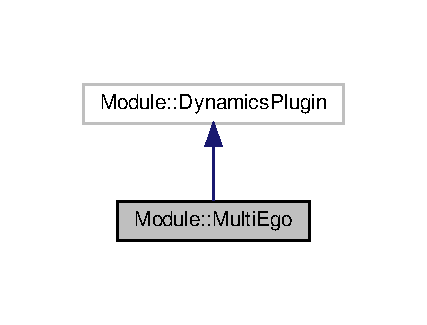
\includegraphics[width=205pt]{classModule_1_1MultiEgo__inherit__graph}
\end{center}
\end{figure}


Collaboration diagram for Module\+:\+:Multi\+Ego\+:\nopagebreak
\begin{figure}[H]
\begin{center}
\leavevmode
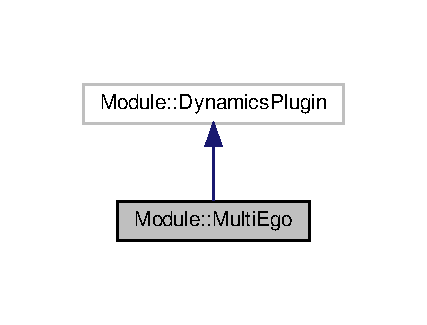
\includegraphics[width=205pt]{classModule_1_1MultiEgo__coll__graph}
\end{center}
\end{figure}
\subsection*{Public Member Functions}
\begin{DoxyCompactItemize}
\item 
\hyperlink{classModule_1_1MultiEgo_a7f19371c1e39db2b07cba0b662bb43f7}{Multi\+Ego} ()
\item 
virtual \hyperlink{classModule_1_1MultiEgo_a6ba87ba21b45b142b48c07cb752c9fa9}{$\sim$\+Multi\+Ego} ()
\item 
virtual bool \hyperlink{classModule_1_1MultiEgo_aa91dec5952b561546ad63bf14517ecc7}{init} ()
\item 
virtual bool \hyperlink{classModule_1_1MultiEgo_ae3c4d04e688fdff789af744205ce6480}{reset} (const double \&sim\+Time)
\item 
virtual int \hyperlink{classModule_1_1MultiEgo_a2bd4f7f6cac18fcf0a1442b58fc5ffe9}{update} (const unsigned long \&frame\+No, Dynamics\+Iface $\ast$iface\+Data)
\item 
virtual bool \hyperlink{classModule_1_1MultiEgo_ad2f951cc83aab77ca8993f1250eb3b69}{handle\+S\+C\+P\+Element} (Framework\+::\+Scp\+Parser $\ast$cmd)
\item 
bool \hyperlink{classModule_1_1MultiEgo_a0f37a737beb2b3be39b4ae081335f61e}{Initialize\+R\+OS} ()
\item 
void \hyperlink{classModule_1_1MultiEgo_a51c4d1e54c327a2c96d2ae60f1d6d1b8}{k\+Throttle\+Pedal\+Callback} (const std\+\_\+msgs\+::\+Float32\+::\+Const\+Ptr \&msg)
\item 
void \hyperlink{classModule_1_1MultiEgo_a9e99889c2f05d5cf14017e114b4fde37}{Reset\+R\+OS} ()
\end{DoxyCompactItemize}
\subsection*{Static Public Member Functions}
\begin{DoxyCompactItemize}
\item 
static Framework\+::\+Plugin $\ast$ \hyperlink{classModule_1_1MultiEgo_afc9e4ee3cf0605085377e1387a2ef16c}{make\+Module} ()
\item 
static void \hyperlink{classModule_1_1MultiEgo_a7a8c8f84f0b814d2340789b119a8598f}{my\+Sigint\+Handler} (int sig)
\end{DoxyCompactItemize}


\subsection{Constructor \& Destructor Documentation}
\mbox{\Hypertarget{classModule_1_1MultiEgo_a7f19371c1e39db2b07cba0b662bb43f7}\label{classModule_1_1MultiEgo_a7f19371c1e39db2b07cba0b662bb43f7}} 
\index{Module\+::\+Multi\+Ego@{Module\+::\+Multi\+Ego}!Multi\+Ego@{Multi\+Ego}}
\index{Multi\+Ego@{Multi\+Ego}!Module\+::\+Multi\+Ego@{Module\+::\+Multi\+Ego}}
\subsubsection{\texorpdfstring{Multi\+Ego()}{MultiEgo()}}
{\footnotesize\ttfamily Module\+::\+Multi\+Ego\+::\+Multi\+Ego (\begin{DoxyParamCaption}{ }\end{DoxyParamCaption})\hspace{0.3cm}{\ttfamily [explicit]}}

constructor \mbox{\Hypertarget{classModule_1_1MultiEgo_a6ba87ba21b45b142b48c07cb752c9fa9}\label{classModule_1_1MultiEgo_a6ba87ba21b45b142b48c07cb752c9fa9}} 
\index{Module\+::\+Multi\+Ego@{Module\+::\+Multi\+Ego}!````~Multi\+Ego@{$\sim$\+Multi\+Ego}}
\index{````~Multi\+Ego@{$\sim$\+Multi\+Ego}!Module\+::\+Multi\+Ego@{Module\+::\+Multi\+Ego}}
\subsubsection{\texorpdfstring{$\sim$\+Multi\+Ego()}{~MultiEgo()}}
{\footnotesize\ttfamily Module\+::\+Multi\+Ego\+::$\sim$\+Multi\+Ego (\begin{DoxyParamCaption}{ }\end{DoxyParamCaption})\hspace{0.3cm}{\ttfamily [virtual]}}

Destroy the class. 

\subsection{Member Function Documentation}
\mbox{\Hypertarget{classModule_1_1MultiEgo_ad2f951cc83aab77ca8993f1250eb3b69}\label{classModule_1_1MultiEgo_ad2f951cc83aab77ca8993f1250eb3b69}} 
\index{Module\+::\+Multi\+Ego@{Module\+::\+Multi\+Ego}!handle\+S\+C\+P\+Element@{handle\+S\+C\+P\+Element}}
\index{handle\+S\+C\+P\+Element@{handle\+S\+C\+P\+Element}!Module\+::\+Multi\+Ego@{Module\+::\+Multi\+Ego}}
\subsubsection{\texorpdfstring{handle\+S\+C\+P\+Element()}{handleSCPElement()}}
{\footnotesize\ttfamily bool Module\+::\+Multi\+Ego\+::handle\+S\+C\+P\+Element (\begin{DoxyParamCaption}\item[{Framework\+::\+Scp\+Parser $\ast$}]{cmd }\end{DoxyParamCaption})\hspace{0.3cm}{\ttfamily [virtual]}}

Reads Module\+Manager.\+xml and also simulation S\+CP 
\begin{DoxyParams}{Parameters}
{\em cmd} & scp commands \\
\hline
\end{DoxyParams}
\begin{DoxyReturn}{Returns}
return success/failure 
\end{DoxyReturn}
\mbox{\Hypertarget{classModule_1_1MultiEgo_aa91dec5952b561546ad63bf14517ecc7}\label{classModule_1_1MultiEgo_aa91dec5952b561546ad63bf14517ecc7}} 
\index{Module\+::\+Multi\+Ego@{Module\+::\+Multi\+Ego}!init@{init}}
\index{init@{init}!Module\+::\+Multi\+Ego@{Module\+::\+Multi\+Ego}}
\subsubsection{\texorpdfstring{init()}{init()}}
{\footnotesize\ttfamily bool Module\+::\+Multi\+Ego\+::init (\begin{DoxyParamCaption}{ }\end{DoxyParamCaption})\hspace{0.3cm}{\ttfamily [virtual]}}

initialize interface \begin{DoxyReturn}{Returns}
success/failure 
\end{DoxyReturn}
\mbox{\Hypertarget{classModule_1_1MultiEgo_a0f37a737beb2b3be39b4ae081335f61e}\label{classModule_1_1MultiEgo_a0f37a737beb2b3be39b4ae081335f61e}} 
\index{Module\+::\+Multi\+Ego@{Module\+::\+Multi\+Ego}!Initialize\+R\+OS@{Initialize\+R\+OS}}
\index{Initialize\+R\+OS@{Initialize\+R\+OS}!Module\+::\+Multi\+Ego@{Module\+::\+Multi\+Ego}}
\subsubsection{\texorpdfstring{Initialize\+R\+O\+S()}{InitializeROS()}}
{\footnotesize\ttfamily bool Module\+::\+Multi\+Ego\+::\+Initialize\+R\+OS (\begin{DoxyParamCaption}{ }\end{DoxyParamCaption})}

Ros initilize function \begin{DoxyReturn}{Returns}
return void 
\end{DoxyReturn}
\mbox{\Hypertarget{classModule_1_1MultiEgo_a51c4d1e54c327a2c96d2ae60f1d6d1b8}\label{classModule_1_1MultiEgo_a51c4d1e54c327a2c96d2ae60f1d6d1b8}} 
\index{Module\+::\+Multi\+Ego@{Module\+::\+Multi\+Ego}!k\+Throttle\+Pedal\+Callback@{k\+Throttle\+Pedal\+Callback}}
\index{k\+Throttle\+Pedal\+Callback@{k\+Throttle\+Pedal\+Callback}!Module\+::\+Multi\+Ego@{Module\+::\+Multi\+Ego}}
\subsubsection{\texorpdfstring{k\+Throttle\+Pedal\+Callback()}{kThrottlePedalCallback()}}
{\footnotesize\ttfamily void Module\+::\+Multi\+Ego\+::k\+Throttle\+Pedal\+Callback (\begin{DoxyParamCaption}\item[{const std\+\_\+msgs\+::\+Float32\+::\+Const\+Ptr \&}]{msg }\end{DoxyParamCaption})}

Handle an incoming ros throttle callback message 
\begin{DoxyParams}{Parameters}
{\em msg} & the incoming message \\
\hline
\end{DoxyParams}
\begin{DoxyReturn}{Returns}
return success/failure 
\end{DoxyReturn}
\mbox{\Hypertarget{classModule_1_1MultiEgo_afc9e4ee3cf0605085377e1387a2ef16c}\label{classModule_1_1MultiEgo_afc9e4ee3cf0605085377e1387a2ef16c}} 
\index{Module\+::\+Multi\+Ego@{Module\+::\+Multi\+Ego}!make\+Module@{make\+Module}}
\index{make\+Module@{make\+Module}!Module\+::\+Multi\+Ego@{Module\+::\+Multi\+Ego}}
\subsubsection{\texorpdfstring{make\+Module()}{makeModule()}}
{\footnotesize\ttfamily static Framework\+::\+Plugin$\ast$ Module\+::\+Multi\+Ego\+::make\+Module (\begin{DoxyParamCaption}{ }\end{DoxyParamCaption})\hspace{0.3cm}{\ttfamily [static]}}

factory function for creating a new object, derived from Param\+Iface \mbox{\Hypertarget{classModule_1_1MultiEgo_a7a8c8f84f0b814d2340789b119a8598f}\label{classModule_1_1MultiEgo_a7a8c8f84f0b814d2340789b119a8598f}} 
\index{Module\+::\+Multi\+Ego@{Module\+::\+Multi\+Ego}!my\+Sigint\+Handler@{my\+Sigint\+Handler}}
\index{my\+Sigint\+Handler@{my\+Sigint\+Handler}!Module\+::\+Multi\+Ego@{Module\+::\+Multi\+Ego}}
\subsubsection{\texorpdfstring{my\+Sigint\+Handler()}{mySigintHandler()}}
{\footnotesize\ttfamily void Module\+::\+Multi\+Ego\+::my\+Sigint\+Handler (\begin{DoxyParamCaption}\item[{int}]{sig }\end{DoxyParamCaption})\hspace{0.3cm}{\ttfamily [static]}}

Signal interupt handler 
\begin{DoxyParams}{Parameters}
{\em sig} & the interupt \\
\hline
\end{DoxyParams}
\begin{DoxyReturn}{Returns}
return void 
\end{DoxyReturn}
\mbox{\Hypertarget{classModule_1_1MultiEgo_ae3c4d04e688fdff789af744205ce6480}\label{classModule_1_1MultiEgo_ae3c4d04e688fdff789af744205ce6480}} 
\index{Module\+::\+Multi\+Ego@{Module\+::\+Multi\+Ego}!reset@{reset}}
\index{reset@{reset}!Module\+::\+Multi\+Ego@{Module\+::\+Multi\+Ego}}
\subsubsection{\texorpdfstring{reset()}{reset()}}
{\footnotesize\ttfamily bool Module\+::\+Multi\+Ego\+::reset (\begin{DoxyParamCaption}\item[{const double \&}]{sim\+Time }\end{DoxyParamCaption})\hspace{0.3cm}{\ttfamily [virtual]}}

reset the plugin (called e.\+g. after re-\/start of simulation) 
\begin{DoxyParams}{Parameters}
{\em sim\+Time} & the simulation time used as reset time \\
\hline
\end{DoxyParams}
\begin{DoxyReturn}{Returns}
true if successful 
\end{DoxyReturn}
\mbox{\Hypertarget{classModule_1_1MultiEgo_a9e99889c2f05d5cf14017e114b4fde37}\label{classModule_1_1MultiEgo_a9e99889c2f05d5cf14017e114b4fde37}} 
\index{Module\+::\+Multi\+Ego@{Module\+::\+Multi\+Ego}!Reset\+R\+OS@{Reset\+R\+OS}}
\index{Reset\+R\+OS@{Reset\+R\+OS}!Module\+::\+Multi\+Ego@{Module\+::\+Multi\+Ego}}
\subsubsection{\texorpdfstring{Reset\+R\+O\+S()}{ResetROS()}}
{\footnotesize\ttfamily void Module\+::\+Multi\+Ego\+::\+Reset\+R\+OS (\begin{DoxyParamCaption}{ }\end{DoxyParamCaption})}

This function reset the ros params \begin{DoxyReturn}{Returns}
void 
\end{DoxyReturn}
\mbox{\Hypertarget{classModule_1_1MultiEgo_a2bd4f7f6cac18fcf0a1442b58fc5ffe9}\label{classModule_1_1MultiEgo_a2bd4f7f6cac18fcf0a1442b58fc5ffe9}} 
\index{Module\+::\+Multi\+Ego@{Module\+::\+Multi\+Ego}!update@{update}}
\index{update@{update}!Module\+::\+Multi\+Ego@{Module\+::\+Multi\+Ego}}
\subsubsection{\texorpdfstring{update()}{update()}}
{\footnotesize\ttfamily int Module\+::\+Multi\+Ego\+::update (\begin{DoxyParamCaption}\item[{const unsigned long \&}]{frame\+No,  }\item[{Dynamics\+Iface $\ast$}]{iface\+Data }\end{DoxyParamCaption})\hspace{0.3cm}{\ttfamily [virtual]}}

handle an incoming dynamics message 
\begin{DoxyParams}{Parameters}
{\em frame\+No} & the current frame number \\
\hline
{\em iface\+Data} & dynamics interface data \\
\hline
\end{DoxyParams}
\begin{DoxyReturn}{Returns}
return code 
\end{DoxyReturn}


The documentation for this class was generated from the following files\+:\begin{DoxyCompactItemize}
\item 
multi\+\_\+ego/inc/Multi\+Ego.\+hh\item 
multi\+\_\+ego/src/Multi\+Ego.\+cc\end{DoxyCompactItemize}

%--- End generated contents ---

% Index
\backmatter
\newpage
\phantomsection
\clearemptydoublepage
\addcontentsline{toc}{chapter}{Index}
\printindex

\end{document}
